\documentclass[10pt, aspectratio=169]{beamer}

% --- THEMES AND COLORS ---
\usetheme{Boadilla}
\usecolortheme{seahorse}

% --- PACKAGES ---
\usepackage[utf8]{inputenc}
\usepackage{graphicx}
\usepackage{booktabs}
\usepackage{amsmath}
\usepackage{pgfplots}
\usepackage{tikz}
\usetikzlibrary{positioning}
\pgfplotsset{compat=1.18}
\usepackage{tabularx}
\usepackage{float}

% --- CUSTOM COLORS (from Guidelines) ---
\definecolor{primaryblue}{HTML}{003399}
\definecolor{accentgreen}{HTML}{2E8B57}
\definecolor{alertred}{HTML}{CC3333}
\definecolor{neutralgray}{HTML}{666666}

\setbeamercolor{structure}{fg=primaryblue}
\setbeamercolor{alerted text}{fg=alertred}
\setbeamercolor{example text}{fg=accentgreen}

% --- TITLE PAGE METADATA ---
\title[Hand Gesture Recognition]{Hand Gesture Recognition for\\Interactive Puzzle Game Control}
\subtitle{A Comparative Analysis of Heuristic, Classical ML, and Neural Network Approaches}
\author[Team]{
    Dinh Thanh Hieu (22BA13132) \and 
    Nguyen Thai Nhat Anh (23BI14024) \and 
    Le Quoc Anh (23BI14025)
}
\institute[USTH]{
    \textbf{Instructor:} Prof. Nguyen Duc Dung \\
    Vietnam Academy of Science and Technology \\
    University of Science and Technology of Hanoi \\[0.5cm]
    
\includegraphics[width=3cm]{usth_logo.png}
}
\date{February 2026}

\begin{document}

% --- SLIDE 1: TITLE ---
\begin{frame}
    \titlepage
\end{frame}

% --- SLIDE 2: PROBLEM STATEMENT ---
\begin{frame}{Motivation: Toward Natural Human-Computer Interaction}
    \begin{itemize}
        \item \textbf{The Core Problem:} Traditional input devices (keyboard, mouse) impose a barrier between user intent and system response. The physical necessity of moving hands off a task to utilize a peripheral disrupts immersive workflows.
        \item \textbf{The Solution:} Hand gestures offer an intuitive, hardware-free alternative by tracking spatial intent directly through a standard webcam.
        \item \textbf{The Engineering Challenge:} Hand morphology varies wildly across users (size, joint flexibility, skin tone). Illumination and viewing angles add massive variance.
        \item \textbf{Research Question:} How can we build a real-time gesture sequence pipeline that generalizes reliably to unseen users without relying on computational-heavy Deep Neural Networks solely?
    \end{itemize}
\end{frame}

% --- SLIDE 3: RESEARCH OBJECTIVES ---
\begin{frame}{Objectives: Three Methods, One Benchmark}
    \begin{itemize}
        \item \textbf{Objective 1:} Implement and compare three gesture classification methods spanning the complexity spectrum:
        \begin{itemize}
            \item Rule-based heuristic (no training data)
            \item Random Forest (engineered features)
            \item Multi-Layer Perceptron (raw landmark coordinates)
        \end{itemize}
        \item \textbf{Objective 2:} Evaluate all methods using person-aware cross-validation on a large-scale public dataset.
        \item \textbf{Objective 3:} Deploy the highest-performing model in a real-time browser-based application.
    \end{itemize}
    \vspace{0.3cm}
    \centering
    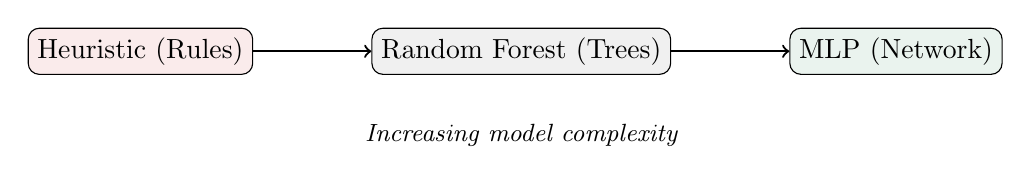
\begin{tikzpicture}
        \node[draw, fill=alertred!10, rounded corners] (h) {Heuristic (Rules)};
        \node[draw, fill=neutralgray!10, rounded corners, right=1.5cm of h] (rf) {Random Forest (Trees)};
        \node[draw, fill=accentgreen!10, rounded corners, right=1.5cm of rf] (mlp) {MLP (Network)};
        \draw[->, thick] (h) -- (rf);
        \draw[->, thick] (rf) -- (mlp);
        \node[below=0.5cm of rf, font=\small\itshape] {Increasing model complexity};
    \end{tikzpicture}
\end{frame}

% --- SLIDE 4: GESTURE VOCABULARY ---
\begin{frame}{Five Gesture Classes, Five Game Actions}
    \centering
    \begin{table}
        \begin{tabular}{@{}lll@{}}
            \toprule
            \textbf{Gesture} & \textbf{Description} & \textbf{Game Action} \\
            \midrule
            Open Hand & Spread fingers, palm forward & Release puzzle piece \\
            Fist & Closed hand & Rotate puzzle piece \\
            Pinch & Thumb and index finger contact & Grab / release piece \\
            Frame & Two hands forming a rectangle & Capture puzzle image \\
            None & No defined gesture & No action \\
            \bottomrule
        \end{tabular}
    \end{table}
\end{frame}

% --- SLIDE 5: SYSTEM ARCHITECTURE ---
\begin{frame}{End-to-End Pipeline: Webcam to Game Control}
    \begin{enumerate}
        \item \textbf{Input Acquisition:} Video frame captured from webcam
        \item \textbf{Landmark Extraction:} Google MediaPipe HandLandmarker produces 21 3D landmarks
        \item \textbf{Normalization:} Position- and scale-invariant preprocessing
        \item \textbf{Classification:} Gesture prediction via one of three evaluated methods
        \item \textbf{Application:} Predicted gesture triggers corresponding game action
    \end{enumerate}
    \vspace{0.3cm}
    \centering
    \textcolor{primaryblue}{
        $\text{Video Frame} \xrightarrow{\text{MediaPipe}} \mathbf{L} \in \mathbb{R}^{21 \times 3} \xrightarrow{\text{Classifier}} y \in \{1,\dots,5\}$
    }
\end{frame}

% --- SLIDE 6: DATASET ---
\begin{frame}{Training Data: The HaGRID v2 Dataset Validation}
    \begin{columns}
        \begin{column}{0.5\textwidth}
            \textbf{Source Dataset Context:}
            \begin{itemize}
                \item Subsampled from \textbf{HaGRID v2} containing over 1 million frames and 37,583 subjects.
                \item Crucial feature: It provides pre-annotated \textbf{2D coordinates $(x,y)$} but depth $z=0.0$, forming an explicit limitation for algorithms relying on 3D geometry.
                \item \textbf{Extraction:} 9,231 stratified samples extracted across 3,607 unique individual identities.
            \end{itemize}
        \end{column}
        \begin{column}{0.5\textwidth}
            \centering
            \begin{table}
                \begin{tabular}{@{}lrrr@{}}
                    \toprule
                    \textbf{Class} & \textbf{Train} & \textbf{Val} & \textbf{Total} \\
                    \midrule
                    open\_hand & 1,000 & 1,000 & 2,000 \\
                    fist & 1,000 & 1,000 & 2,000 \\
                    pinch & 1,000 & 1,000 & 2,000 \\
                    frame & 1,000 & 1,000 & 2,000 \\
                    none & 1,000 & 231 & 1,231 \\
                    \midrule
                    \textbf{Total} & \textbf{5,000} & \textbf{4,231} & \textbf{9,231} \\
                    \bottomrule
                \end{tabular}
            \end{table}
        \end{column}
    \end{columns}
\end{frame}

% --- SLIDE 7: PREPROCESSING ---
\begin{frame}{Feature Extraction: Landmark Normalization Invariance}
    \textbf{Problem:} Raw coordinates break classifiers the moment a user moves away from the camera or shifts their hand. \\
    \vspace{0.3cm}
    \textbf{Solution:} Standardize orientation and scale using a vector pipeline:
    \begin{itemize}
        \item \textbf{Translation Invariance:} We shift the mathematical space so the Wrist (Index 0) acts as coordinates $(0,0)$. This makes model blind to \textit{where} the hand is in the video.
        \item \textbf{Scale Invariance:} We divide coordinates by the Euclidean distance to the Middle Finger joint (Index 9). This makes the model blind to \textit{hand dimension size}.
        \item \textbf{Result:} A pure \textbf{60-dimensional structural vector} per frame (20 joints $\times$ 3 axes).
    \end{itemize}
    \begin{equation*}
        \hat{\mathbf{l}}_i = \frac{\mathbf{l}_i - \mathbf{l}_0}{\|\mathbf{l}_9 - \mathbf{l}_0\|_2}, \quad \text{for } i = 1, \dots, 20
    \end{equation*}
\end{frame}

% --- SLIDE 8: METHOD 1 ---
\begin{frame}{Method 1: Rule-Based Heuristic Classification}
    \begin{columns}
        \begin{column}{0.55\textwidth}
            \begin{itemize}
                \item \textbf{Approach:} $\sim$20 manually calibrated thresholds on finger curl angles and inter-landmark distances.
                \item \textbf{Result:} \textcolor{alertred}{\textbf{0.99\% accuracy}}---below random baseline of 20\%!
                \item \textbf{Reason why this is crucial to present:} It validates our data limitations. The HaGRID dataset is 2D ($z=0$); attempting 3D geometry causes vector calculations to degenerate to random noise. If we had 3D ground truth, Heuristic models would likely perform exceptionally fast.
            \end{itemize}
        \end{column}
        \begin{column}{0.45\textwidth}
            \begin{figure}
                \centering
                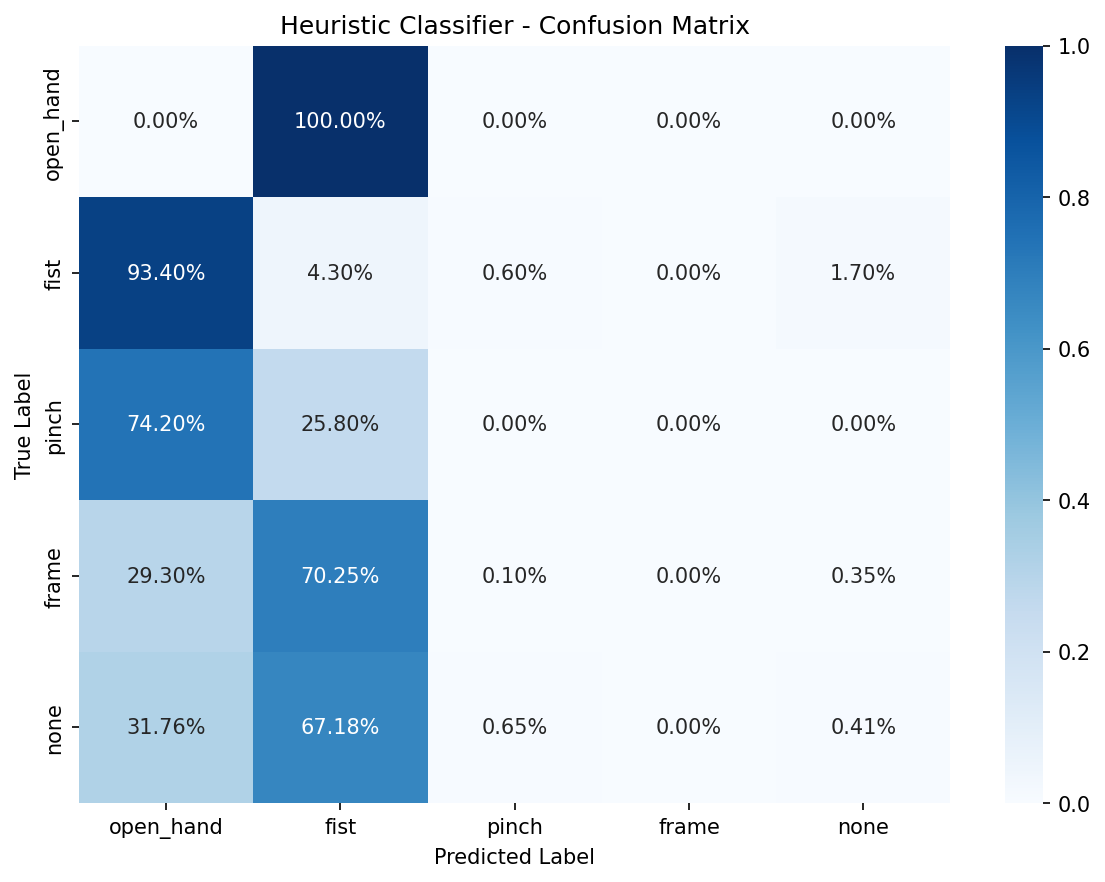
\includegraphics[height=5cm]{models/plots/heuristic_confusion_matrix.png}
            \end{figure}
        \end{column}
    \end{columns}
\end{frame}

% --- SLIDE 9: METHOD 2 ---
\begin{frame}{Method 2: Random Forest with Engineered Features}
    \begin{columns}
        \begin{column}{0.45\textwidth}
            \begin{itemize}
                \item \textbf{Configuration:} 100 Trees (\texttt{max\_depth}=15)
                \item \textbf{Input:} Instead of 60 raw coords, we engineer a condensed 24-dim vector of pairwise Euclidean distances.
                \item \textbf{Result:} \textbf{94.13\% accuracy} (13.2 ms latency).
                \item \textbf{Strength:} Highly interpretable, we can see exactly which distances contribute to choices.
            \end{itemize}
        \end{column}
        \begin{column}{0.55\textwidth}
            \begin{figure}
                \centering
                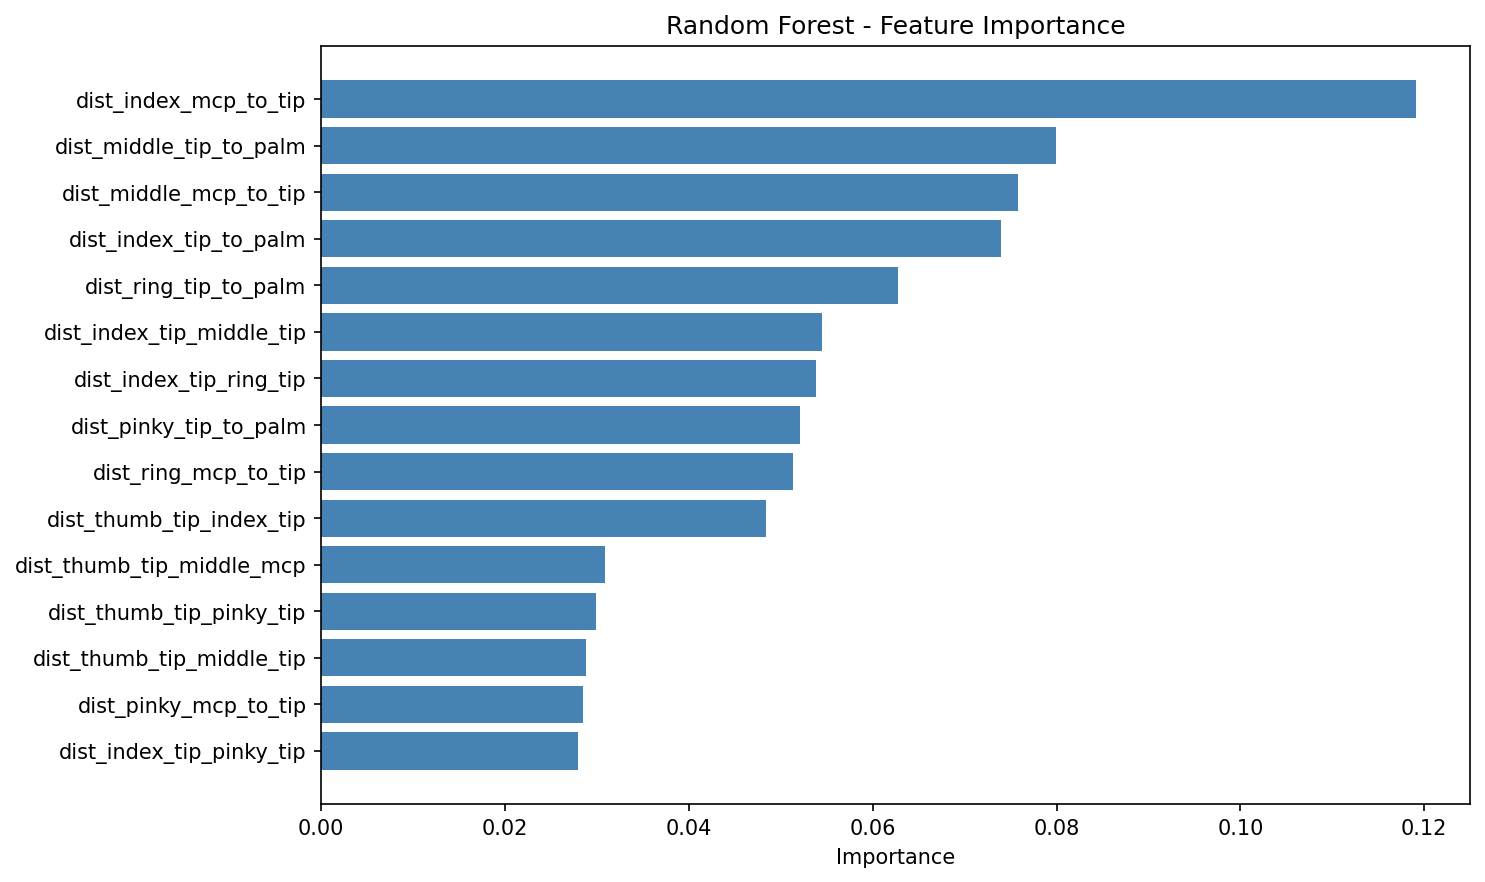
\includegraphics[width=\textwidth, height=6.5cm, keepaspectratio]{models/plots/rf_feature_importance.png}
            \end{figure}
        \end{column}
    \end{columns}
\end{frame}

% --- SLIDE 10: METHOD 3 ---
\begin{frame}{Method 3: Multi-Layer Perceptron on Raw Landmarks}
    \begin{columns}
        \begin{column}{0.5\textwidth}
            \begin{itemize}
                \item \textbf{Architecture:} A 2-Hidden-Layer Network ($60 \rightarrow 128 \rightarrow 64 \rightarrow 5$) with Dropout regularization.
                \item \textbf{Size:} Barely 14,789 parameters (227 KB footprint).
                \item \textbf{Result:} Peak \textcolor{accentgreen}{\textbf{98.41\% accuracy}}, 43.7 ms inference latency. No feature engineering needed.
            \end{itemize}
        \end{column}
        \begin{column}{0.5\textwidth}
            \begin{figure}
                \centering
                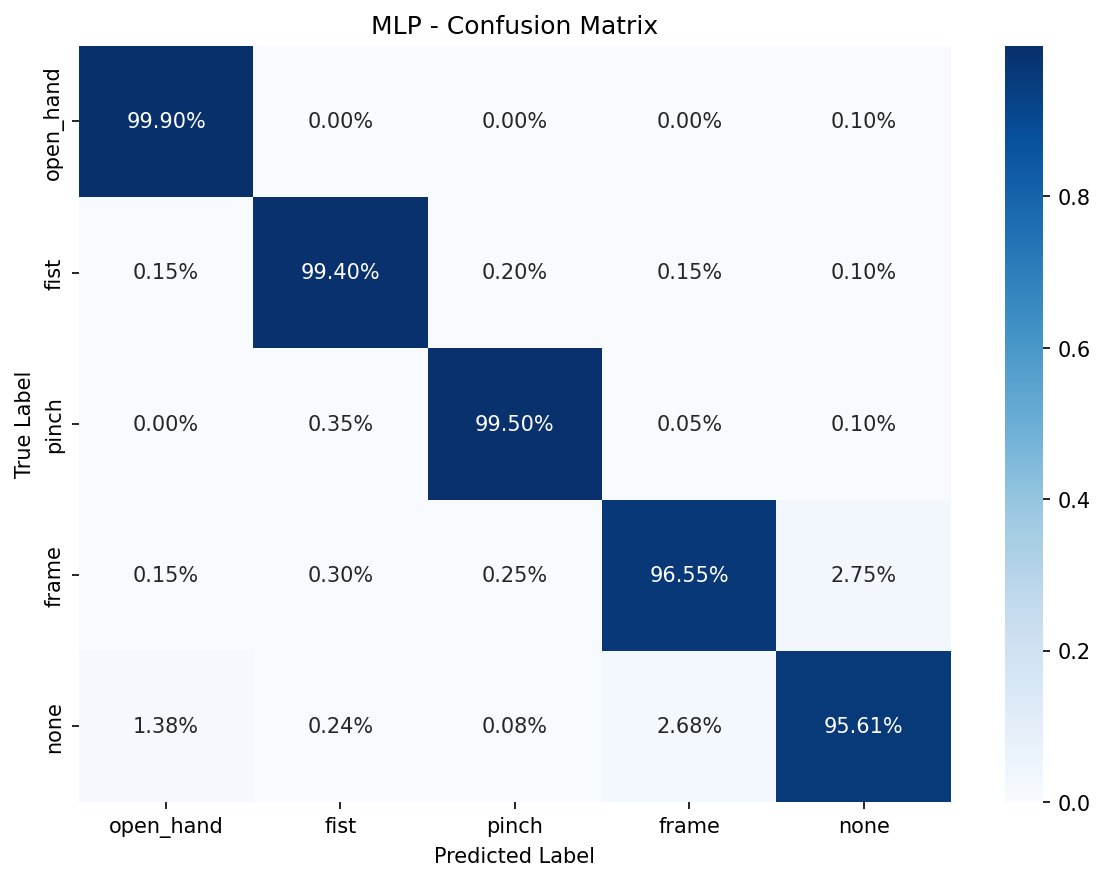
\includegraphics[width=\textwidth, height=5.5cm, keepaspectratio]{models/plots/mlp_confusion_matrix.png}
            \end{figure}
        \end{column}
    \end{columns}
\end{frame}

% --- SLIDE 11: SUMMARY TABLE ---
\begin{frame}{Three Methods: Head-to-Head Comparison}
    \centering
    \begin{table}
        \small
        \begin{tabular}{@{}llll@{}}
            \toprule
            \textbf{Criterion} & \textbf{Heuristic} & \textbf{Random Forest} & \textbf{MLP} \\
            \midrule
            Input & Angles + dist. & 24 pairwise dist. & 60 raw coords \\
            Feature Eng. & Manual & Semi-automatic & None (end-to-end) \\
            Training & No & Yes & Yes \\
            Parameters & $\sim$20 thresholds & $\sim$100K nodes & 14,789 weights \\
            Model Size & \textcolor{accentgreen}{170 B} & 8.6 MB & 227 KB \\
            \midrule
            CV Accuracy & \textcolor{alertred}{0.99\%} & 94.13\% & \textcolor{accentgreen}{\textbf{98.41\%}} \\
            Latency & \textcolor{accentgreen}{0.1 ms} & 13.2 ms & 43.7 ms \\
            \bottomrule
        \end{tabular}
    \end{table}
\end{frame}

% --- SLIDE 12: EVALUATION METHODOLOGY ---
\begin{frame}{Person-Aware Cross-Validation: Ensuring Generalization}
    \begin{itemize}
        \item \textbf{Method:} Group 5-Fold Cross-Validation with person IDs as group identifiers.
        \item \textbf{Guarantee:} No individual appears in both training and test partitions within any fold.
        \item \textbf{Rationale:} Standard random splits risk identity leakage---the model may memorize individual hand morphology rather than learning gesture geometry.
        \item \textbf{Scale:} 3,607 unique subjects ensure diversity in hand shape, skin tone, and gesture style.
    \end{itemize}
\end{frame}

% --- SLIDE 13: ACCURACY VS LATENCY ---
\begin{frame}{The Accuracy-Latency Tradeoff}
    \begin{columns}
        \begin{column}{0.5\textwidth}
            \begin{itemize}
                \item \textbf{Heuristic:} 0.99\% at 0.1 ms -- fast but non-functional
                \item \textbf{Random Forest:} 94.13\% at 13.2 ms -- within 60 FPS budget (16.7 ms threshold)
                \item \textbf{MLP:} 98.41\% at 43.7 ms -- highest accuracy, rate $\sim$23 FPS
                \item \textit{Interactive limit:} 23 FPS is sufficient for gesture transitions which occur at human speed ($\sim$1--2 per sec).
            \end{itemize}
        \end{column}
        \begin{column}{0.5\textwidth}
            \begin{figure}
                \centering
                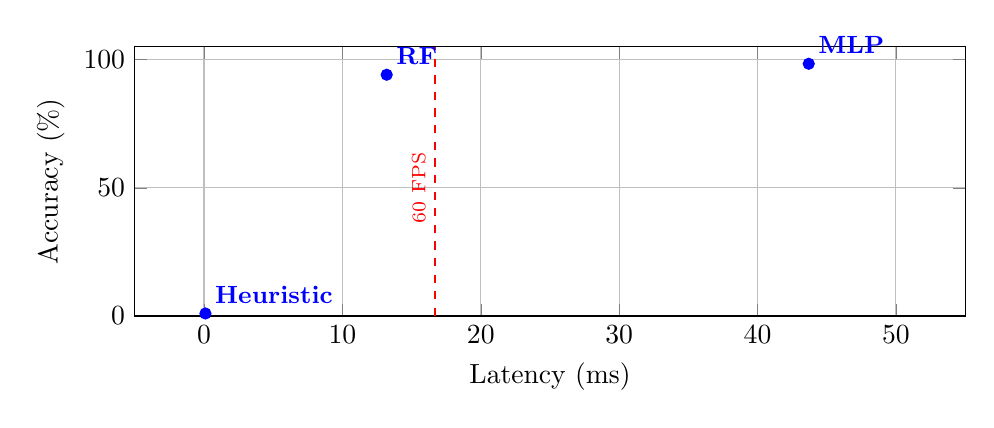
\begin{tikzpicture}
                    \begin{axis}[
                        width=\textwidth, height=5cm,
                        xlabel={Latency (ms)},
                        ylabel={Accuracy (\%)},
                        xmin=-5, xmax=55, ymin=0, ymax=105,
                        grid=major,
                        nodes near coords, nodes near coords style={font=\small\bfseries, anchor=south west},
                        point meta=explicit symbolic,
                    ]
                    \addplot[only marks, mark=*, blue] coordinates {
                        (0.1, 0.99) [Heuristic]
                        (13.2, 94.13) [RF]
                        (43.7, 98.41) [MLP]
                    };
                    \draw[dashed, red, thick] (axis cs:16.7, 0) -- (axis cs:16.7, 105);
                    \node[rotate=90, anchor=south, red] at (axis cs:16.7, 50) {\scriptsize 60 FPS};
                    \end{axis}
                \end{tikzpicture}
            \end{figure}
        \end{column}
    \end{columns}
\end{frame}

% --- SLIDE 14: ERROR ANALYSIS ---
\begin{frame}{Error Distribution: Where Do Models Fail?}
    \begin{itemize}
        \item \textbf{Random Forest:} Two-handed "Frame" gesture loses context since joints are processed per hand (F1 = 89.2\%).
        \item \textbf{MLP Correction:} Fixes inter-hand context dropping, restoring Frame F1 to 97.3\% (an \textbf{8.1\% bump}).
    \end{itemize}
    \vspace{0.3cm}
    \begin{columns}
        \begin{column}{0.48\textwidth}
            \centering
            \textbf{Random Forest}\\
            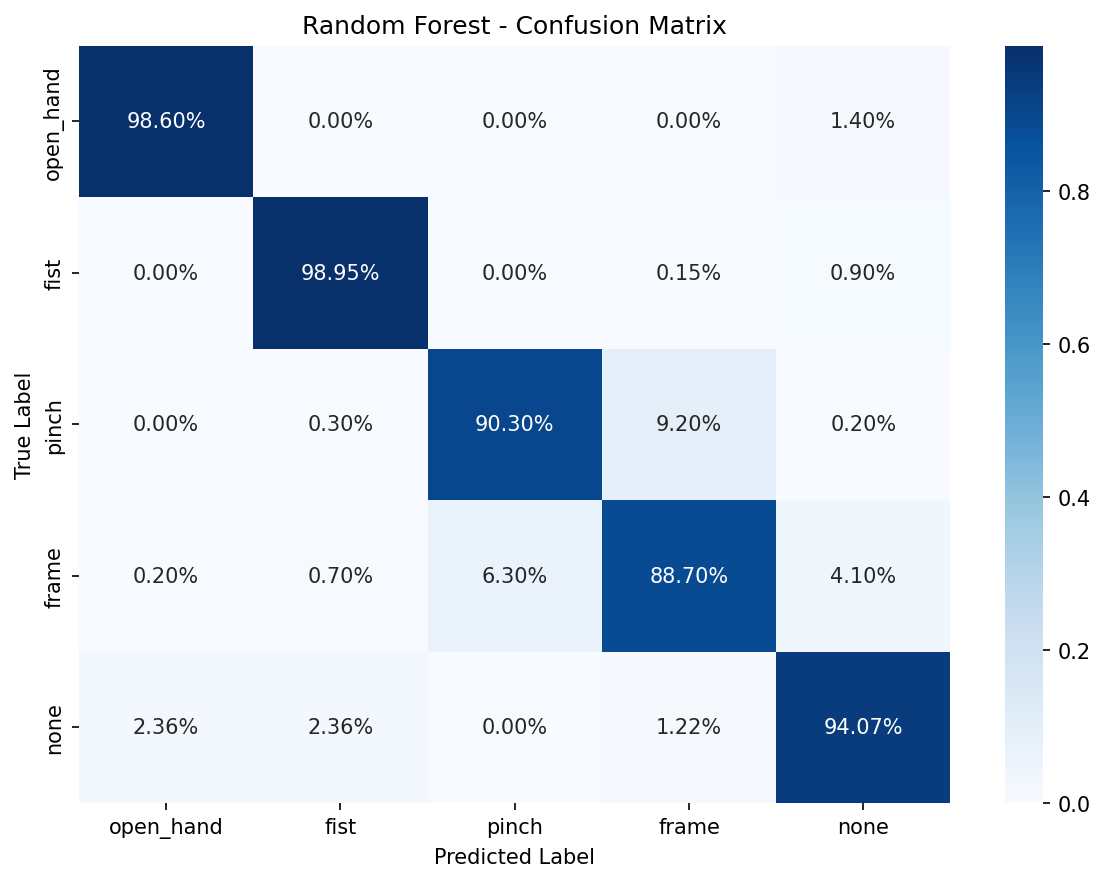
\includegraphics[height=4.5cm]{models/plots/rf_confusion_matrix.png}
        \end{column}
        \begin{column}{0.04\textwidth}
            \centering \Huge $\rightarrow$
        \end{column}
        \begin{column}{0.48\textwidth}
            \centering
            \textbf{MLP}\\
            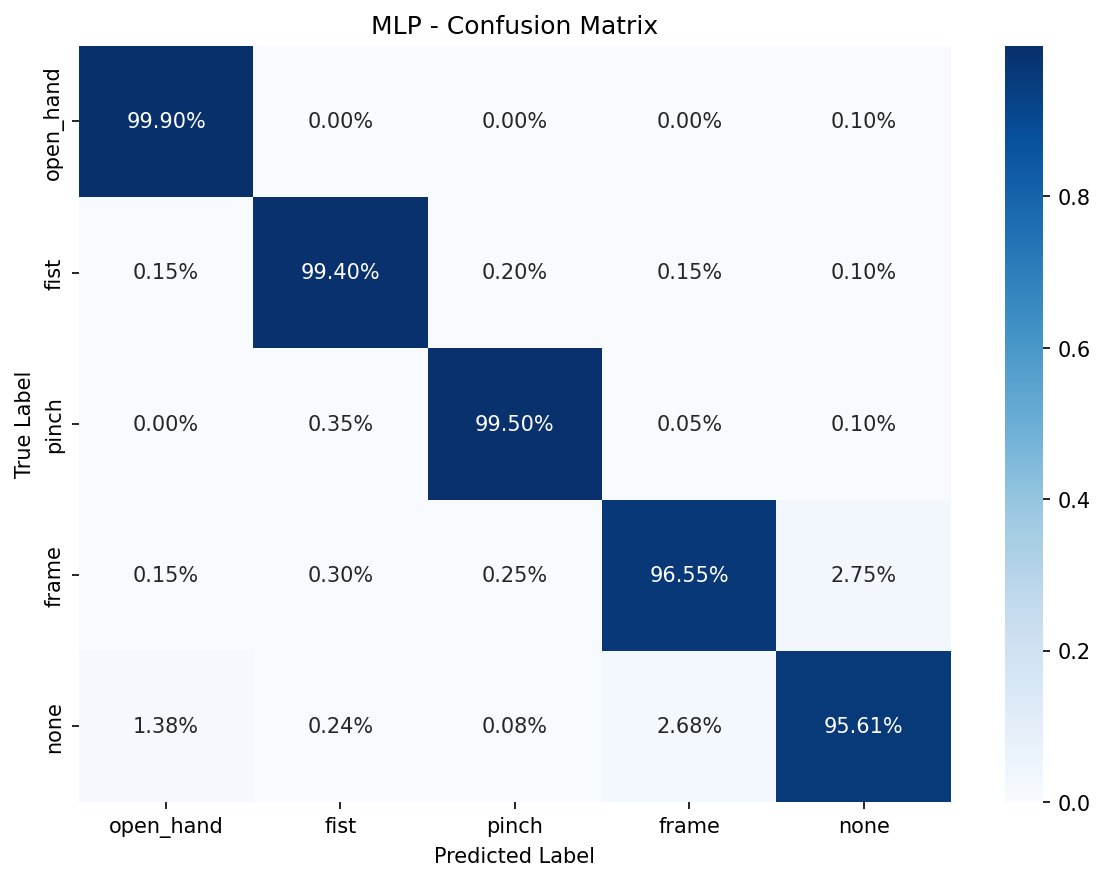
\includegraphics[height=4.5cm]{models/plots/mlp_confusion_matrix.png}
        \end{column}
    \end{columns}
\end{frame}

% --- SLIDE 15: PER-CLASS F1 SCORES ---
\begin{frame}{Per-Class F1 Scores: MLP Advantage Across All Categories}
    \begin{columns}
        \begin{column}{0.5\textwidth}
            \begin{table}
                \small
                \begin{tabular}{@{}lllc@{}}
                    \toprule
                    \textbf{Class} & \textbf{RF F1} & \textbf{MLP F1} & \textbf{Delta} \\
                    \midrule
                    open\_hand & 0.985 & 0.994 & +0.009 \\
                    fist & 0.983 & 0.993 & +0.010 \\
                    pinch & 0.919 & 0.995 & \textbf{+0.076} \\
                    frame & 0.892 & 0.973 & \textbf{+0.081} \\
                    none & 0.919 & 0.953 & +0.034 \\
                    \bottomrule
                \end{tabular}
            \end{table}
        \end{column}
        \begin{column}{0.65\textwidth}
            \begin{figure}
                \centering
                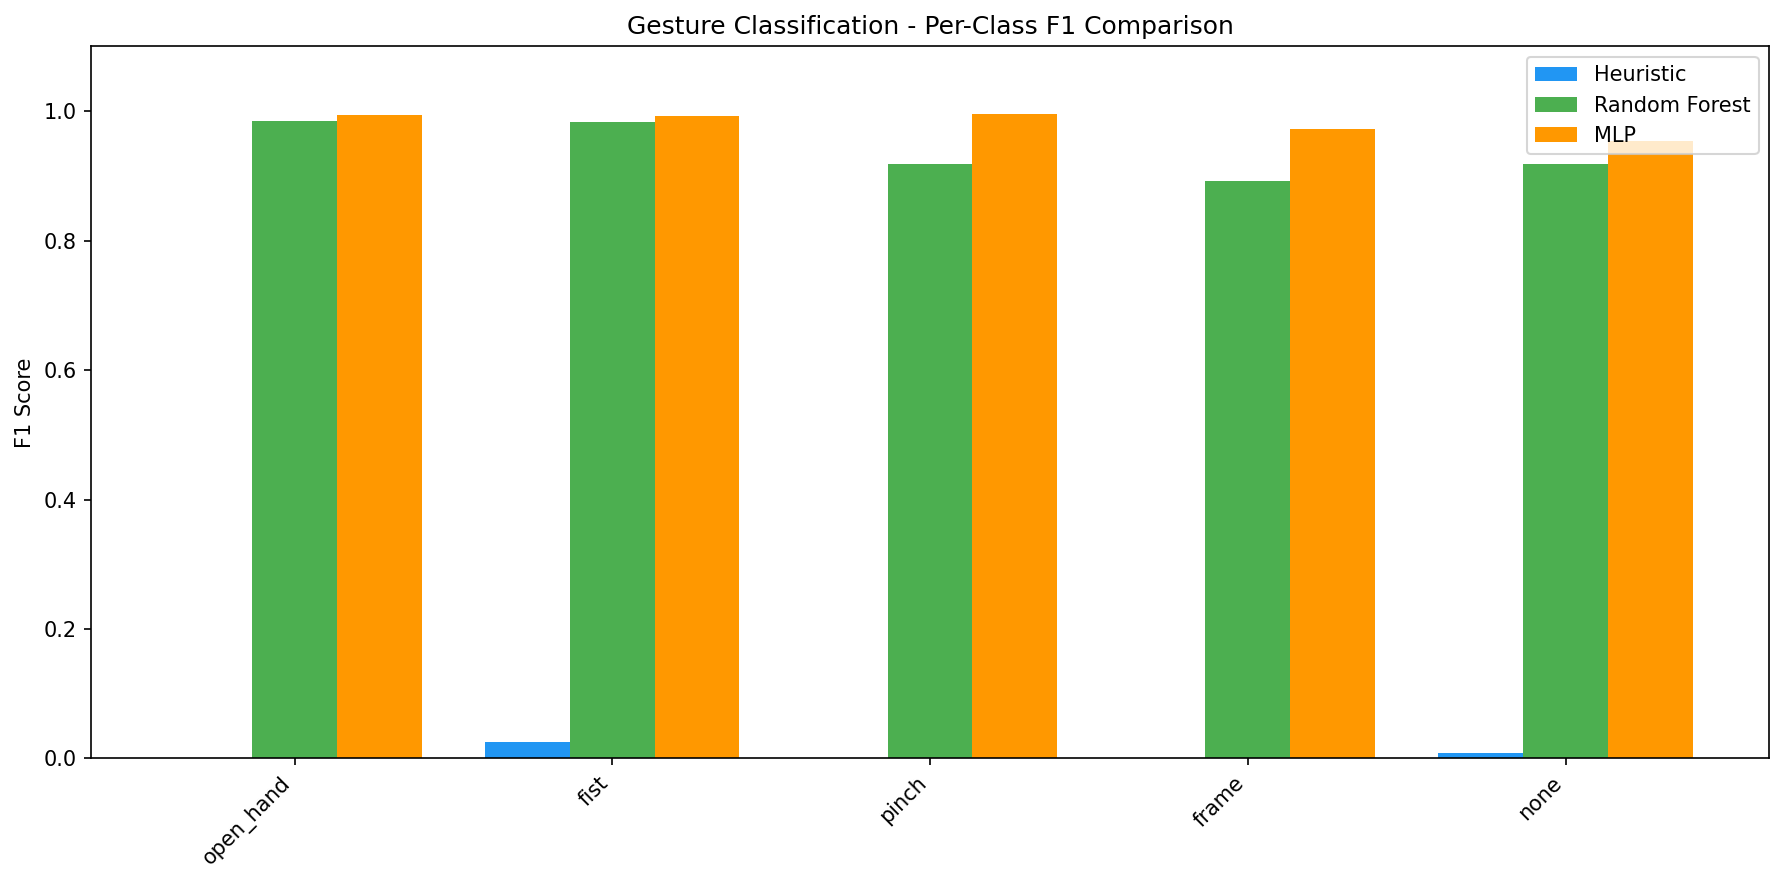
\includegraphics[width=\textwidth, height=6.5cm, keepaspectratio]{models/plots/per_class_f1_comparison.png}
            \end{figure}
        \end{column}
    \end{columns}
\end{frame}

% --- SLIDE 16: CV STABILITY ---
\begin{frame}{Generalization Consistency Across Folds}
    \begin{columns}
        \begin{column}{0.55\textwidth}
            \begin{table}
                \footnotesize
                \begin{tabular}{@{}lccc@{}}
                    \toprule
                    \textbf{Fold} & \textbf{Heuristic} & \textbf{RF} & \textbf{MLP} \\
                    \midrule
                    1 & 0.60\% & 93.45\% & 98.48\% \\
                    2 & 0.98\% & 94.64\% & 97.89\% \\
                    3 & 1.30\% & 94.75\% & 98.54\% \\
                    4 & 1.25\% & 92.09\% & 98.54\% \\
                    5 & 0.81\% & 95.72\% & 98.59\% \\
                    \bottomrule
                \end{tabular}
            \end{table}
        \end{column}
        \begin{column}{0.45\textwidth}
            \begin{itemize}
                \item \textbf{MLP:} std = 0.26\%, invariant to test population.
                \item \textbf{RF:} std = 1.25\% -- fold 4 dip suggests sensitivity to specific subject geometric variations.
            \end{itemize}
        \end{column}
    \end{columns}
\end{frame}

% --- SLIDE 17: DEMONSTRATION ---
\begin{frame}{System Demonstration: Real-Time Gesture-Controlled Puzzle}
    \begin{itemize}
        \item \textbf{Platform:} Browser-based application (HTML5 Canvas, JavaScript ES6)
        \item \textbf{Inference stack:} MediaPipe WASM (landmark detection) + ONNX Runtime Web (MLP classification)
        \item \textbf{Architecture:} Fully client-side -- no backend server, functions offline after initial load.
        \item \textbf{Temporal smoothing:} 3-frame debounce buffer prevents gesture jitter.
    \end{itemize}
    \vspace{0.3cm}
    \centering
    \textit{[Live Demonstration in Class]}
\end{frame}

% --- SLIDE 18: SOFTWARE ENGINEERING ---
\begin{frame}{Implementation Quality: modular Architecture and Testing}
    \begin{itemize}
        \item \textbf{Test coverage:} 28 automated tests spanning preprocessing, feature extraction, classifiers, and data conversion.
        \item \textbf{Modular design:} Single-responsibility modules with clean interfaces.
        \item \textbf{Reproducibility:} Single command executes the full pipeline from data extraction through evaluation.
    \end{itemize}
    \begin{block}{Project Directory}
        \small\texttt{CVsubject/ml/} \\
        \texttt{├── preprocessing.py | features.py | train.py | evaluate.py} \\
        \texttt{├── heuristic.py | random\_forest.py | mlp.py} \\
        \texttt{└── tests/test\_core.py \# 28 automated tests}
    \end{block}
\end{frame}

% --- SLIDE 19: LIMITATIONS & FUTURE ---
\begin{frame}{Current Limitations and Proposed Extensions}
    \begin{columns}
        \begin{column}{0.5\textwidth}
            \textbf{Limitations:}
            \begin{itemize}
                \item Heuristic fails with 2D landmarks.
                \item Frame gesture accuracy impaired by per-hand evaluation.
                \item MLP drops below 60 FPS bound.
            \end{itemize}
        \end{column}
        \begin{column}{0.5\textwidth}
            \textbf{Future Directions:}
            \begin{itemize}
                \item Model quantization (TFLite, ONNX) for WebAssembly.
                \item Two-stage frame detector.
                \item Temporal sequence modeling (LSTM, 1D-CNN).
            \end{itemize}
        \end{column}
    \end{columns}
\end{frame}

% --- SLIDE 20: CONCLUSION ---
\begin{frame}{Summary and Key Findings}
    \begin{itemize}
        \item \textbf{Data-driven superiority:} ML methods outperform heuristics by two orders of magnitude (98\% vs 1\%).
        \item \textbf{Highest Accuracy:} MLP achieves 98.41\% ($\pm$0.26\%) ensuring reliable game interactions.
        \item \textbf{Speed vs. Reliability:} Random Forest meets strict 60 FPS latency constraints but neural networks handle sub-optimal inputs better.
        \item \textbf{Methodology matters:} Person-aware CV prevents reporting inflated accuracies characteristic of identity leakage.
    \end{itemize}
    \vspace{0.4cm}
    \begin{center}
        \begin{quote}
            ``The gap between classical ML and deep learning is incremental (4 points), but the decision must be governed by practical hardware latency constraints.''
        \end{quote}
    \end{center}
\end{frame}

\end{document}
